\chapter{Metodología y método de trabajo}
\label{cap:MiMetodologia}

En este capítulo se explica la metodología de desarrollo que se ha seguido, describiendo desde la captura de requisitos hasta el producto final. Al final del capítulo se añade un apartado con el análisis de costes.

\section{Metodología de desarrollo}

Se ha seguido una metodología de desarrollo en espiral: el \gls{pud}.

\subsection{Características principales}
El \gls{pud} es una metodología de desarrollo que transforma los requisitos de usuario en un sistema software. Es muy genérica, y por eso se ha decidido adaptar a este proyecto.
Las características básicas del \gls{pud} son las siguientes:
\begin{itemize}
	\item \textbf{Dirigido por casos de uso:} en este proyecto, los usuarios, como se ha mencionado anteriormente, son los maestros y profesores de \gls{eso}. Los casos de uso que se han contemplado para el proyecto son las acciones que se han especificado en \ref{cap:Introduccion}. Se hablará de la metodología seguida para la captura de requisitos más adelante.
	\item \textbf{Centrado en la arquitectura:} una de las primeras fases del proyecto es realizar el esquema de la base de datos y la comprensión de la futura arquitectura del programa. Esto determinará el orden en el que se desarrollarán los casos de uso.
	\item \textbf{Iterativo e incremental:} se ha trabajado mediante iteraciones, en la que cada una o bien añadía una nueva funcionalidad, mejoraba una de las ya existentes, o realizaba pruebas de cohesión entre los módulos recién añadidos y los que ya estaban desarrollados. También cabe notar que el método de iteraciones ha sido el de terminar por completo una parte, hasta las pruebas, antes de comenzar con otra nueva. \todo{acordarse de hablar de esto}Esto ha tenido repercusiones de las que se hablarán más adelante. En cada iteración en la que se añade una nueva funcionalidad:
	\begin{enumerate}
		\item Se elige una de las que todavía no se han desarrollado.
		\item Dentro de la funcionalidad, se identifican y especifican los casos de uso que le corresponden.
		\item Se refinan los diseños que se hicieron al principio del proyecto para estos casos de uso.
		\item Se implementan y se prueban dentro del módulo de manera que satisfaga de manera vaga los requisitos.
	\end{enumerate}
	
	En cada iteración en la que se mejora una funcionalidad existente:
	\begin{enumerate}
		\item Se elige una de las funcionalidades a probar.
		\item Se prueba exhaustivamente dentro de su módulo para identificar los errores actuales y posibles futuros, y se arreglan los fallos.
	\end{enumerate}
	
	En cada iteración en la que se prueba la cohesión entre los módulos:
	\begin{enumerate}
		\item Se elige uno de los módulos, preferentemente el último que se ha desarrollado.
		\item Se prueba con el resto de los módulos con los que mantiene cualquier tipo de comunicación, se identifican los errores y se arreglan los fallos.
	\end{enumerate}
	
	\item Enfocado en los riesgos: primero se han desarrollado los casos de uso más grandes que, después del primer diseño, se consideró que tendrían más impacto en el programa. Seguidamente, se fue trabajando desarrollando los distintos módulos, uno por cada funcionalidad y una iteración por funcionalidad.
	
\end{itemize}


Esta metodología consiste en la división del proyecto en cuatro etapas:
\begin{itemize}
    \item \textbf{Inicio:} para comenzar, se recogerán todos los requisitos y se estimará el alcance del proyecto.
    \item \textbf{Elaboración:} se harán prototipos de las interfaces, se diseñará el software mediante diagramas y se estimarán las iteraciones a seguir.
    \item \textbf{Construcción:} se escribirá el software según el resultado de la fase de elaboración, siguiendo las iteraciones previamente calculadas. 
    \item \textbf{Transición:} para finalizar se probará el producto final y, si procede, se dará fin al desarrollo.
\end{itemize}


Para la obtención y clasificación de los requisitos, se optará por varias metodologías:
\begin{itemize}
	\item \textbf{Observación activa:} se estudiará el entorno de trabajo del usuario final. Para ello, se realizó una sesión en la que se monitorizó a un usuario usando una de las herramientas descritas en el capítulo Aplicaciones existentes, preguntándole sus opiniones sobre algunas de las características que estaba utilizando.
	\item \textbf{Entrevistas:} entrevistas con el usuario en las que irá evaluando el producto final de cada sprint y añadiendo o modificando características.
\end{itemize}

Además, se ha usado la regla MoSCoW para priorizar el desarrollo de los requisitos. Esta regla divide los requisitos en cuatro categorías:
\begin{enumerate}
	\item \textbf{Must have (M):} requisitos que la aplicación debe tener y son prioritarios a cualquier otro de menor rango. Estos requisitos se consideraron en esta categoría:
	\begin{itemize}
		\item Creación de tareas.
		\item Calificación de tareas.
		\item Visualización de las notas del alumnado.
	\end{itemize}
	
	
	\item \textbf{Should have (S):} estos requisitos, de menor rango que los Must have, siguen siendo requisitos importantes para el desarrollo de la aplicación. Estos se consideró que fueran:
	\begin{itemize}
		\item Visualización de informes del alumno.
		\item Visualización de informes del curso.
	\end{itemize}
	
	
	\item \textbf{Could have (C):} requisitos de más baja prioridad, que pueden posponerse si hay otros de mayor rango por encima de ellos.  Estos requisitos han sido:
	\begin{itemize}
		\item Sistema de inicio de sesión para el maestro.
		\item Modificación de los datos del maestro.
	\end{itemize}
	
	
	\item \textbf{Won't have (W):} requisitos completamente opcionales que la aplicación podría llegar a tener de manera que mejorasen las funcionalidades.
	\begin{itemize}
		\item Exportación a Excel de las notas del alumnado.
		\item Creación y asignación de alumnos/as a un curso o a una asignatura.
		\item Estadísticas de las notas del alumnado.
		\item Informaciones adicionales sobre las notas del alumnado.
		\item Sugerencias personalizadas para el usuario.
	\end{itemize}
	
	
\end{enumerate}

	
\section{Prototipos de interfaces}
En las figuras \ref{Fig:mockup_mainwindow}, \ref{Fig:mockup_nuevatarea} y \ref{Fig:mockup_informealumno} se muestran algunos de los prototipos que se hicieron en la fase de elaboración para las interfaces del programa.

\begin{figure}[h]
\centering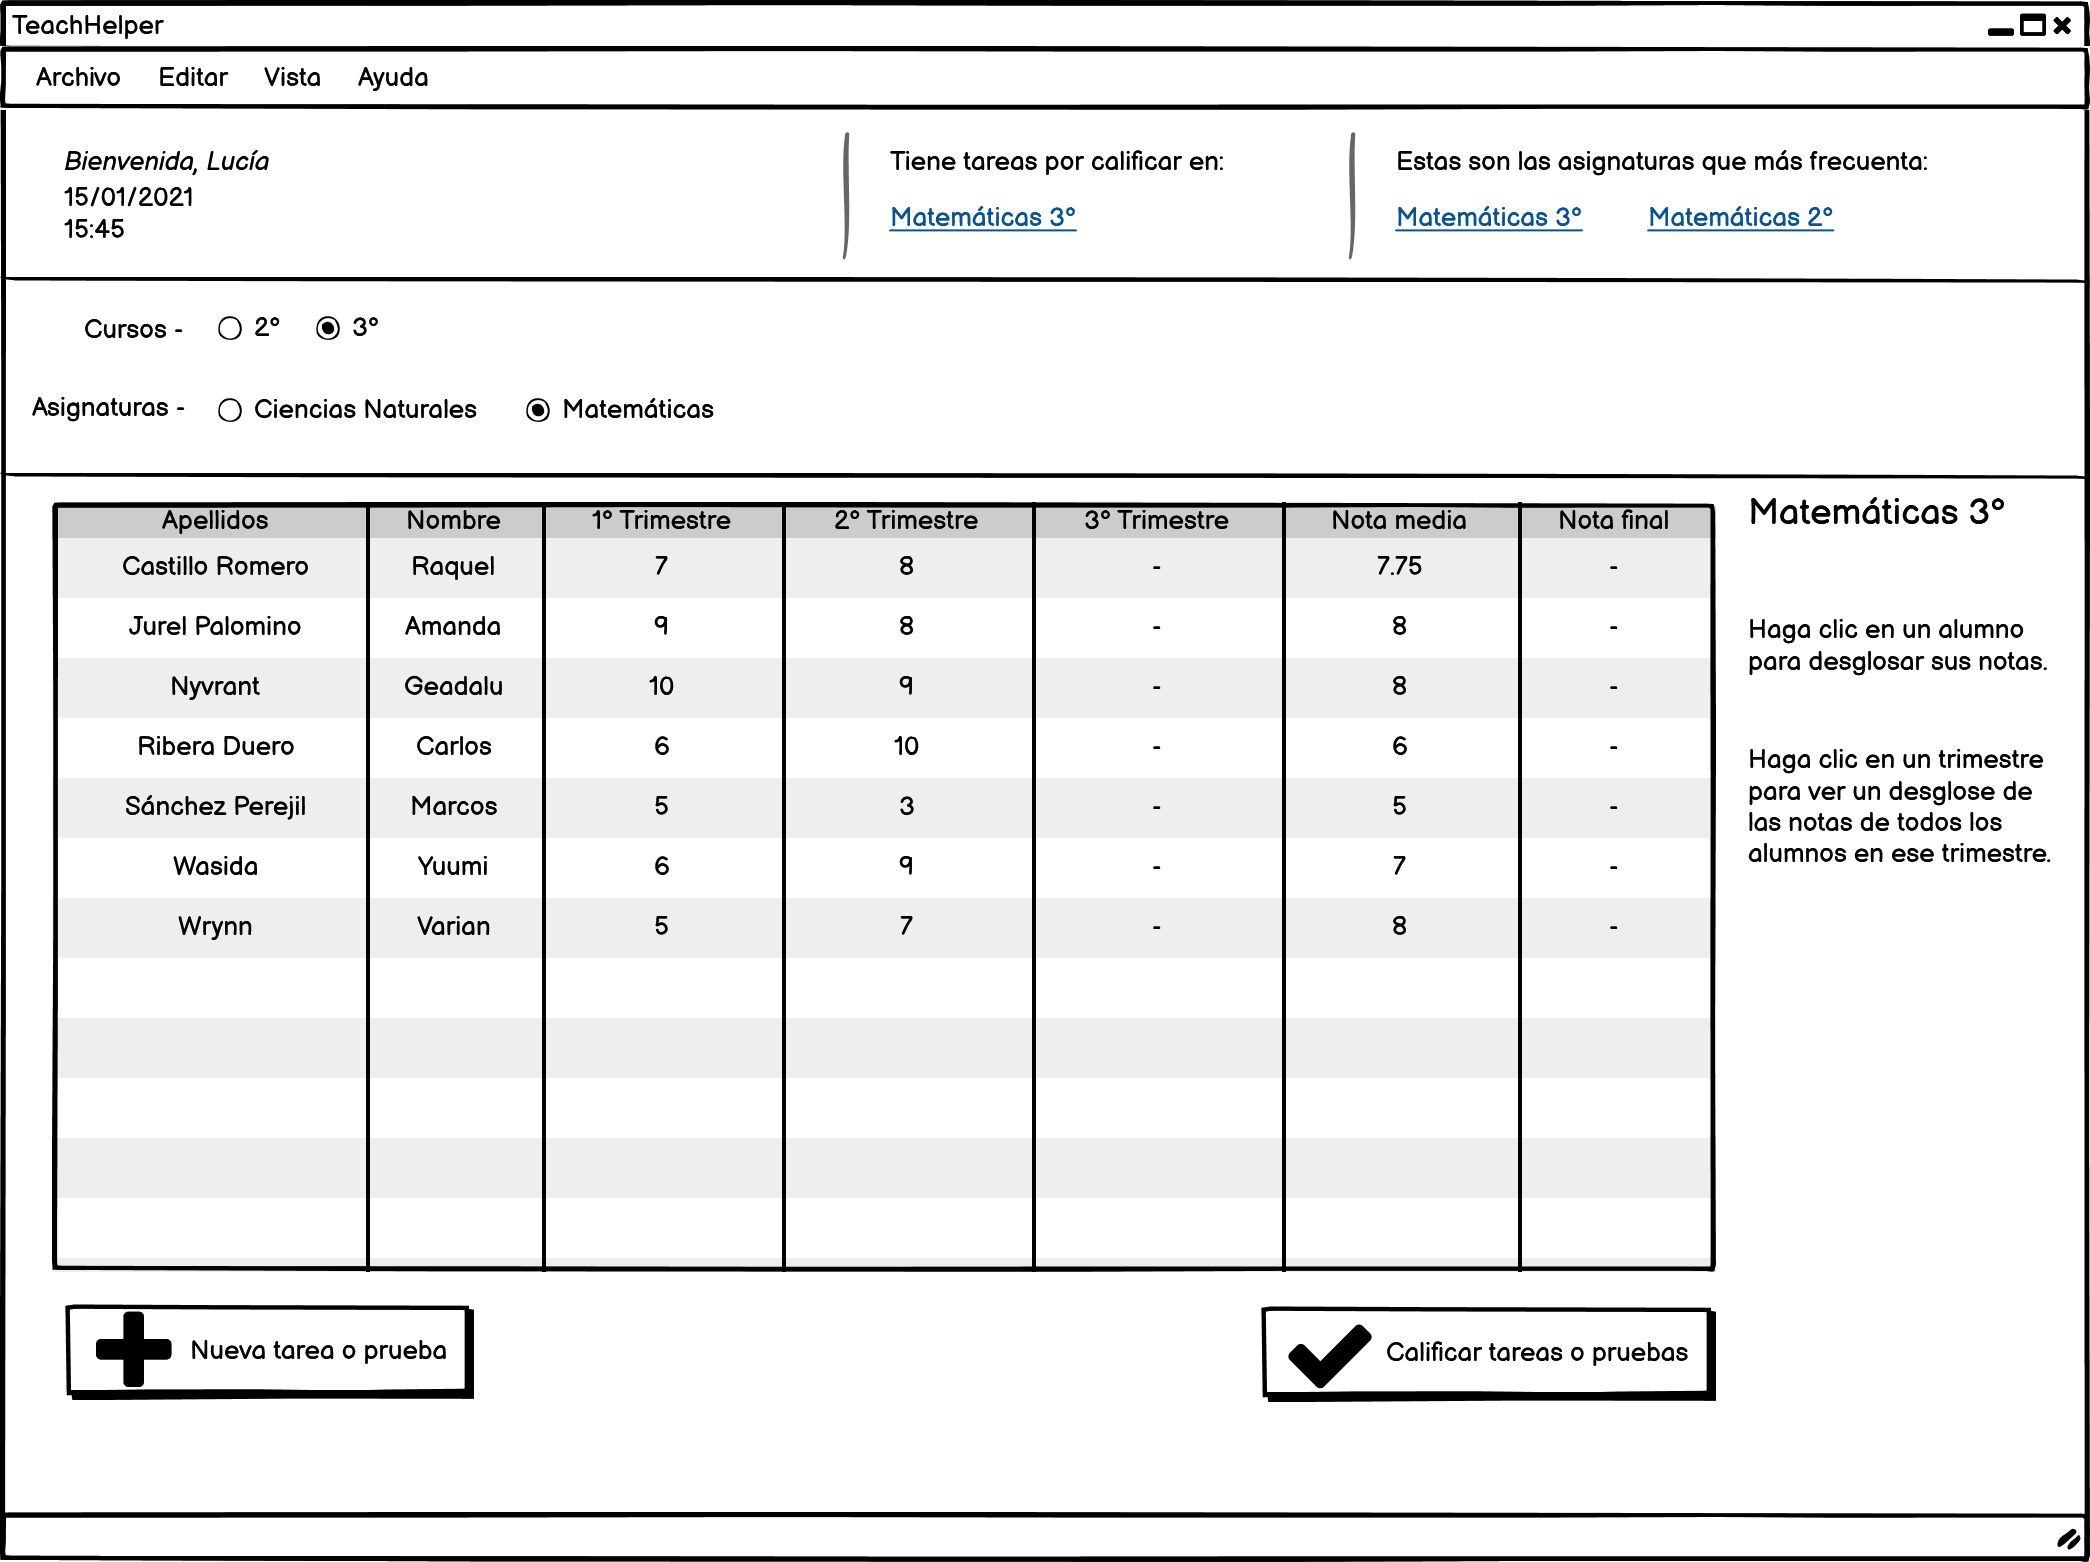
\includegraphics[width=1\linewidth]{figs/mockup_mainwindow.png}
\caption{Ventana principal.}
\label{Fig:mockup_mainwindow}
\end{figure}

\begin{figure}[h]
\centering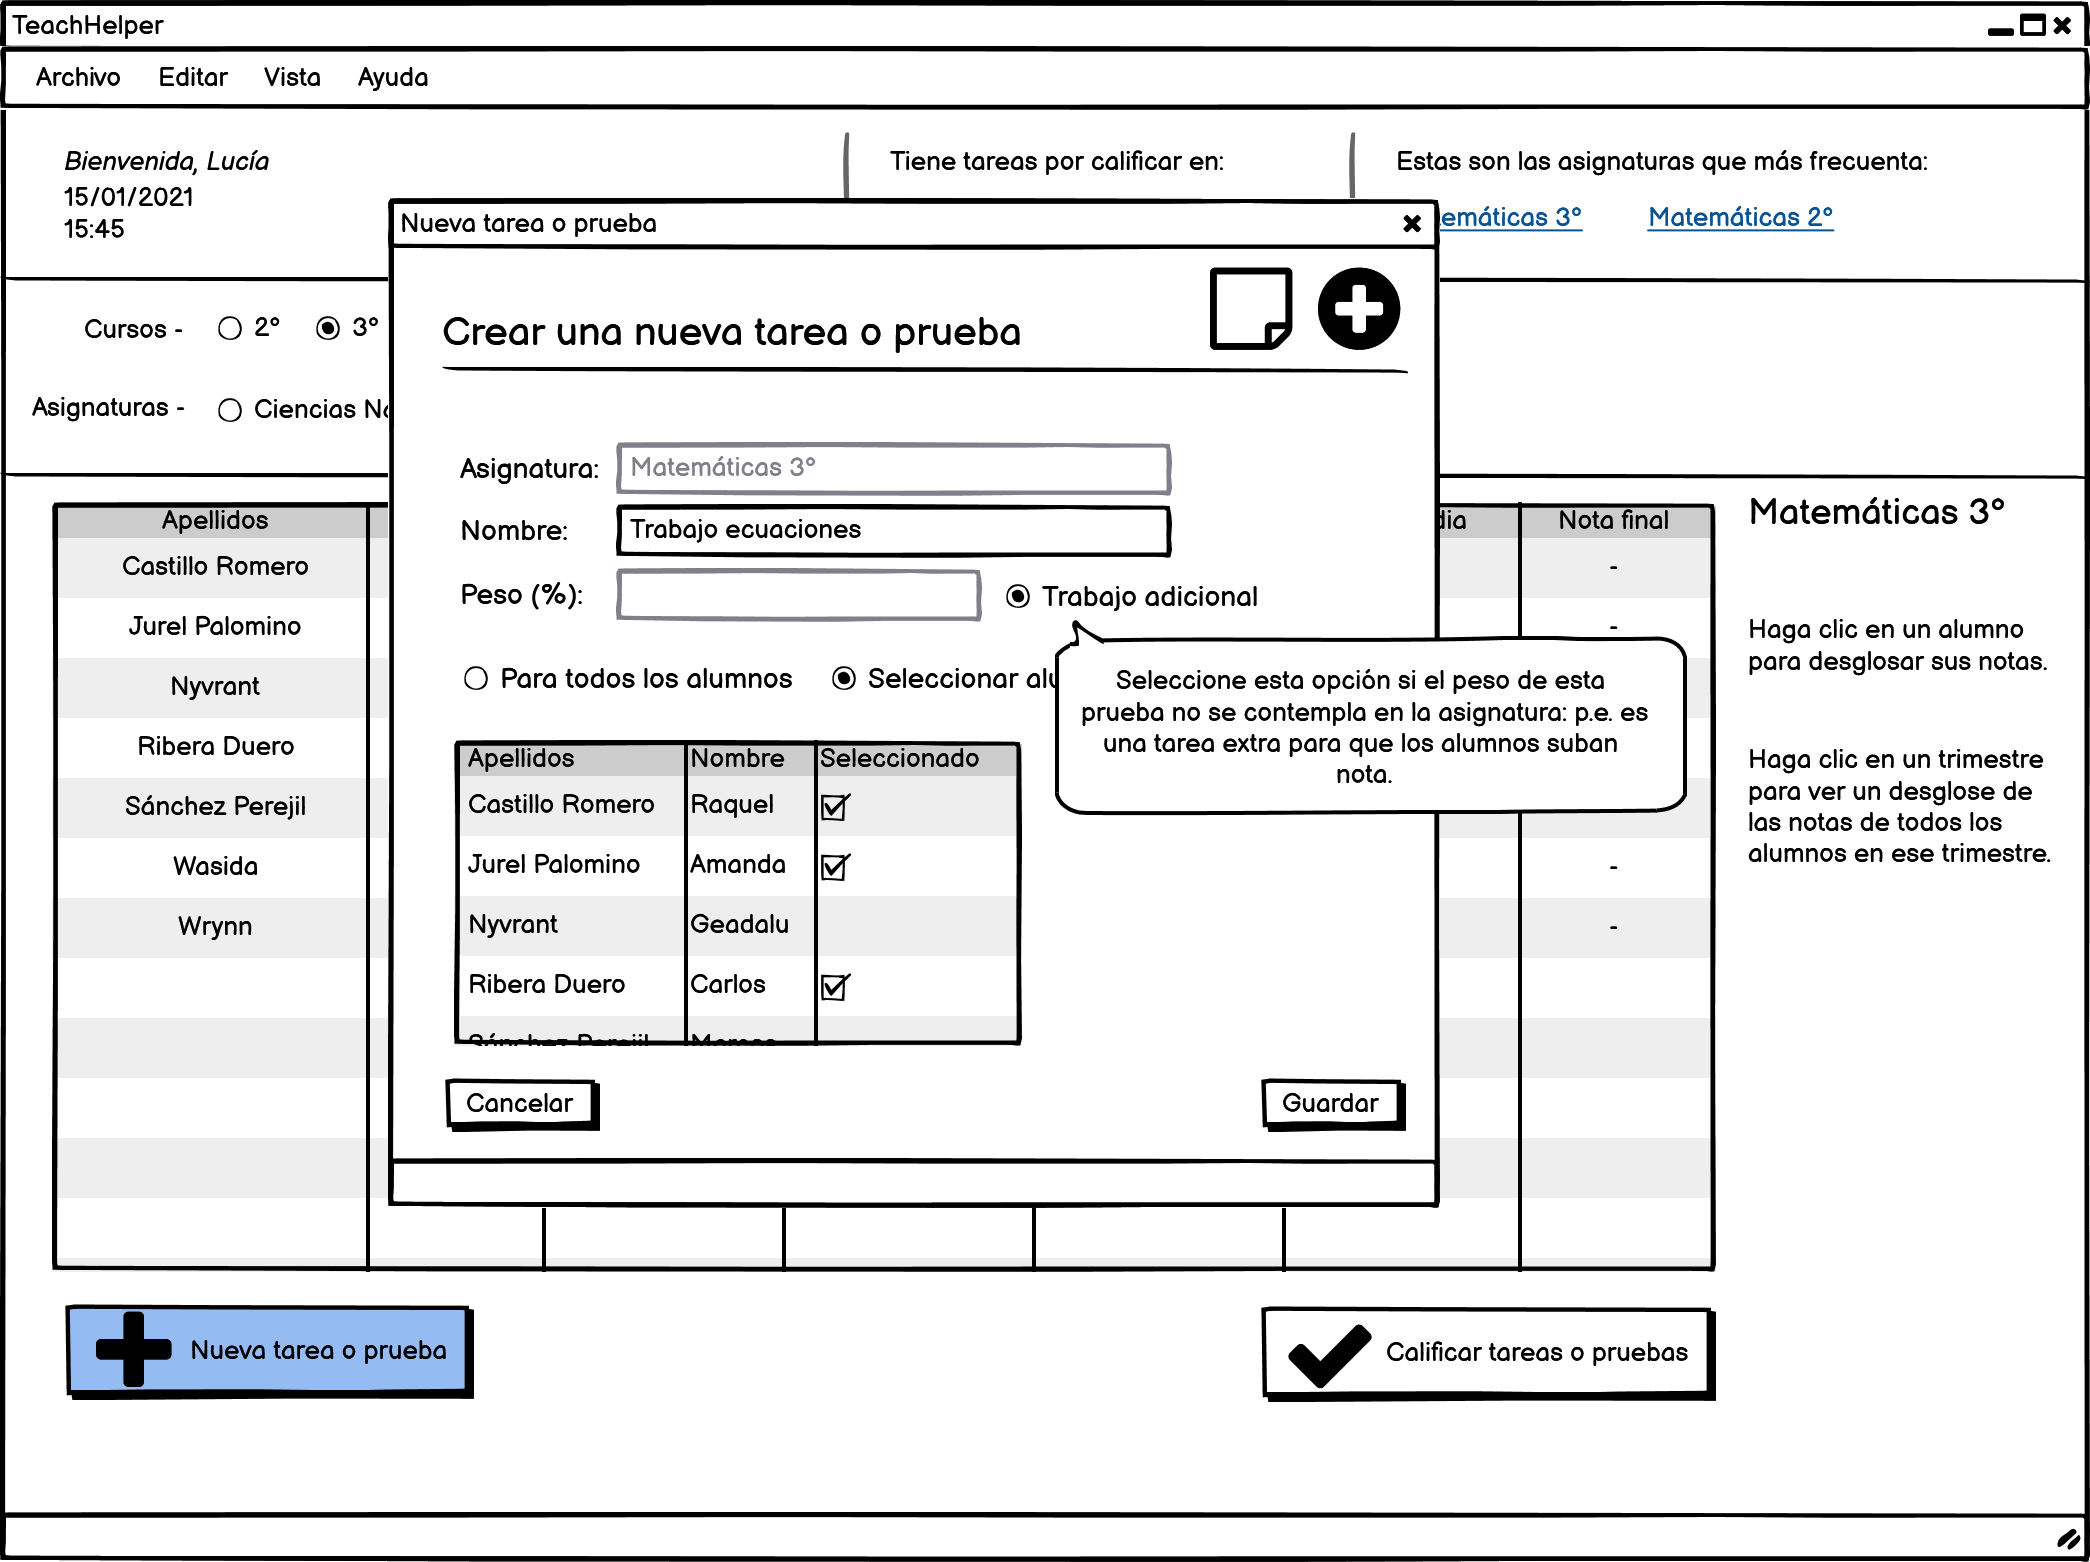
\includegraphics[width=1\linewidth]{figs/mockup_nuevatarea.png}
\caption{Crear nuevas tareas o pruebas.}
\label{Fig:mockup_nuevatarea}
\end{figure}

\begin{figure}[h]
\centering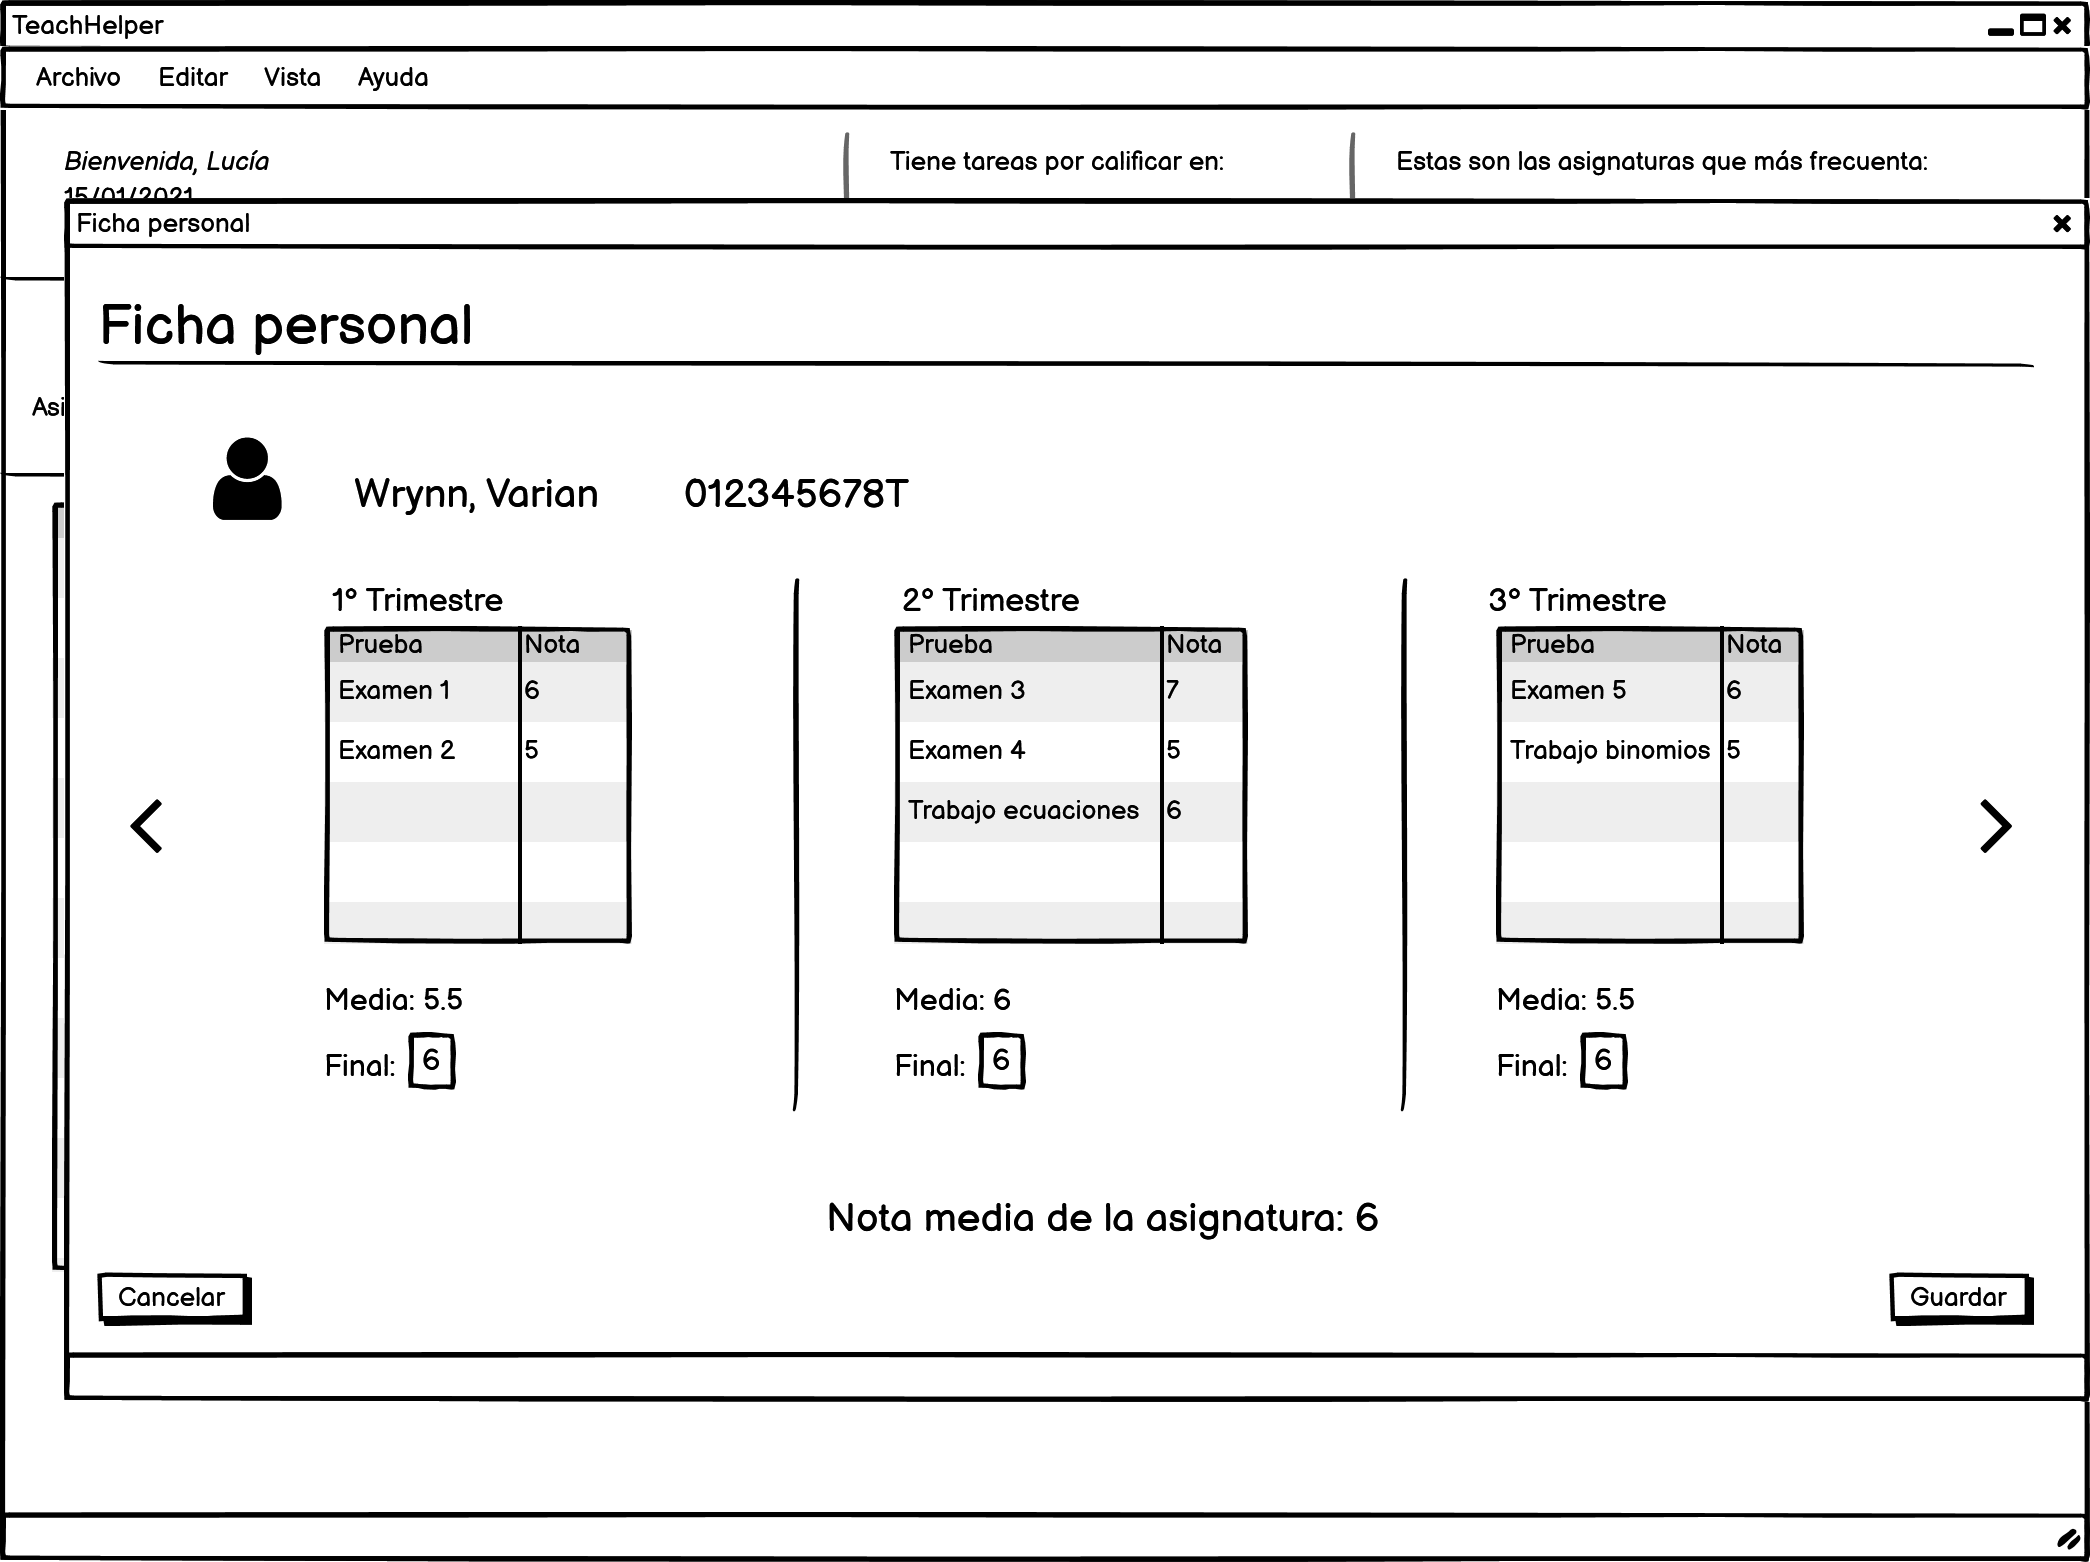
\includegraphics[width=1\linewidth]{figs/mockup_informealumno.png}
\caption{Informe del alumnado.}
\label{Fig:mockup_informealumno}
\end{figure}




\section{Sprints}


\subsection{Primer sprint - 2oct/1nov}

En el primer sprint (2 octubre 2020 - 1 noviembre 2020) se realizaron los diseños de la aplicación con la herramienta Balsamiq Wireframes. Estos diseños han ido cambiando varias veces a lo largo de este primer sprint. Además, se realizó el primer diseño de la base de datos (ver figura \ref{Fig:db_definition1}).

\begin{figure}[h]
\centering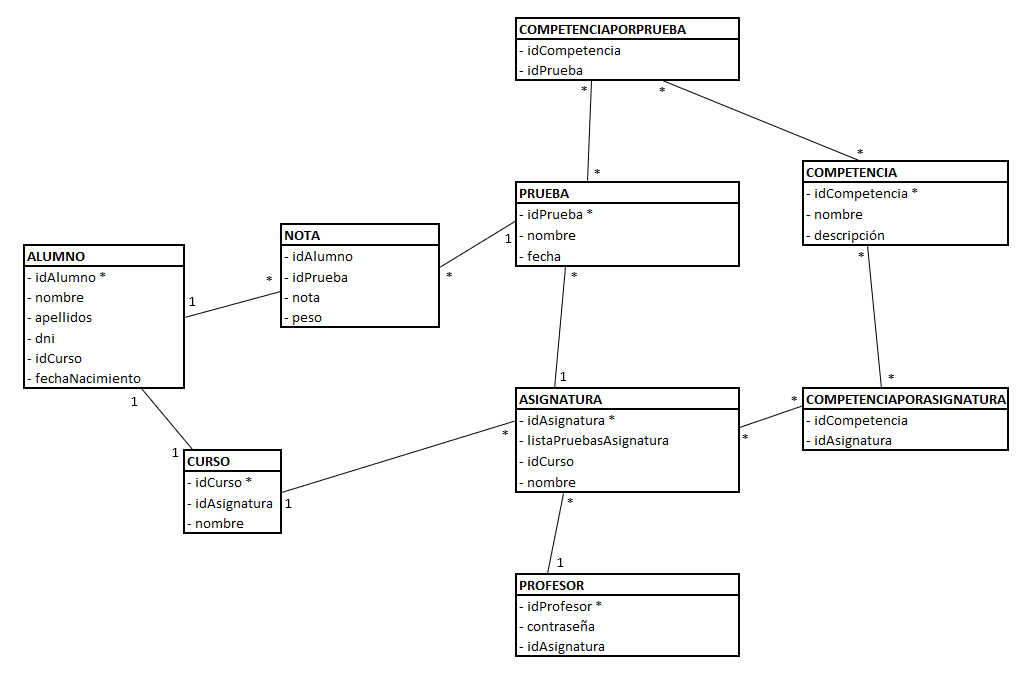
\includegraphics[width=1\linewidth]{figs/DB_Definition_1.png}
\caption{Primera definición de la base de datos.}
\label{Fig:db_definition1}
\end{figure}

\subsection{Segundo sprint - 2nov/1dic}

En el segundo sprint (2 noviembre 2020 - 1 diciembre 2020) se hicieron los siguientes cambios:
\begin{itemize}
	\item Comienzo de la escritura de la memoria del trabajo
	\item Implementación de la base de datos
\end{itemize}

\subsection{Tercer sprint - 2dic/1ene}

En el tercer sprint (2 diciembre 2020 - 1 febrero 2021) se hicieron los siguientes cambios:
\begin{itemize}
	\item Comienzo de la implementación de la aplicación: creación de la ventana principal.
	\item Se pobla inicialmente la base de datos con datos de prueba.
\end{itemize}

\subsection{Cuarto sprint - 2feb/1mar}

En el cuarto sprint (2 febrero 2021 - 1 marzo 2021) se continuó con el desarrollo de la ventana principal. Cabe notar que en este sprint se decidió dejar las mejoras del diseño de la ventana para sprints posteriores y comenzar con el desarrollo de las funcionalidades.

\subsection{Quinto sprint - 2mar/1may}

En el quinto sprint (2 marzo 2021 - 1 abril 2021) se continuó con el desarrollo general de la aplicación.

\subsection{Sexto sprint - 2may/1jul}

El sexto sprint (2 mayo 2021 - 1 julio 2021) se dedicó a corregir y realizar pequeños desarrollos en la aplicación, que si bien no añadían nuevas funcionalidades, pulían las ya existentes.

